\section{Methodology Overview}

The general processing steps for the project can be grouped into four
processing stages. A simplified overview of these staged and the flow
of data between them is shown in Figure \ref{fig:simple-work}. In
ascending order, each processing stage is discussed in more detail in
Sections \ref{met:seq-workflow}, \ref{met:predict-workflow},
\ref{met:valid-workflow}, and .

\begin{figure}
  \centering
  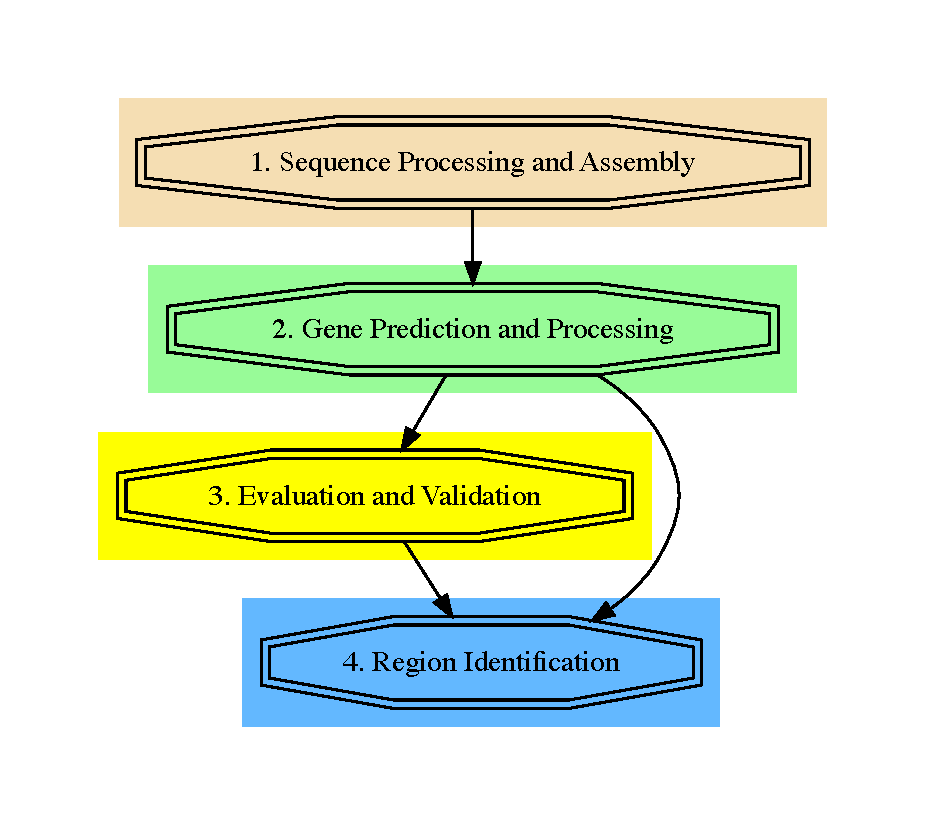
\includegraphics[width=0.8\textwidth]{figures/workflow-simple.pdf}
  \caption{A simplified workflow used in this work. Each processing
    stage is is represented by an octagon, and data flows are
    indicated by directed edges between them. In this figure and
    subsequent figures, the sequence processing stage is colored
    brown, the gene prediction and processing stage is colored green,
    the evaluation and validation stage is colored yellow, and the
    region identification process is colored blue.}
  \label{fig:simple-work}
\end{figure}

%\begin{figure}
%  \centering
%  \makebox[0pt]{
%    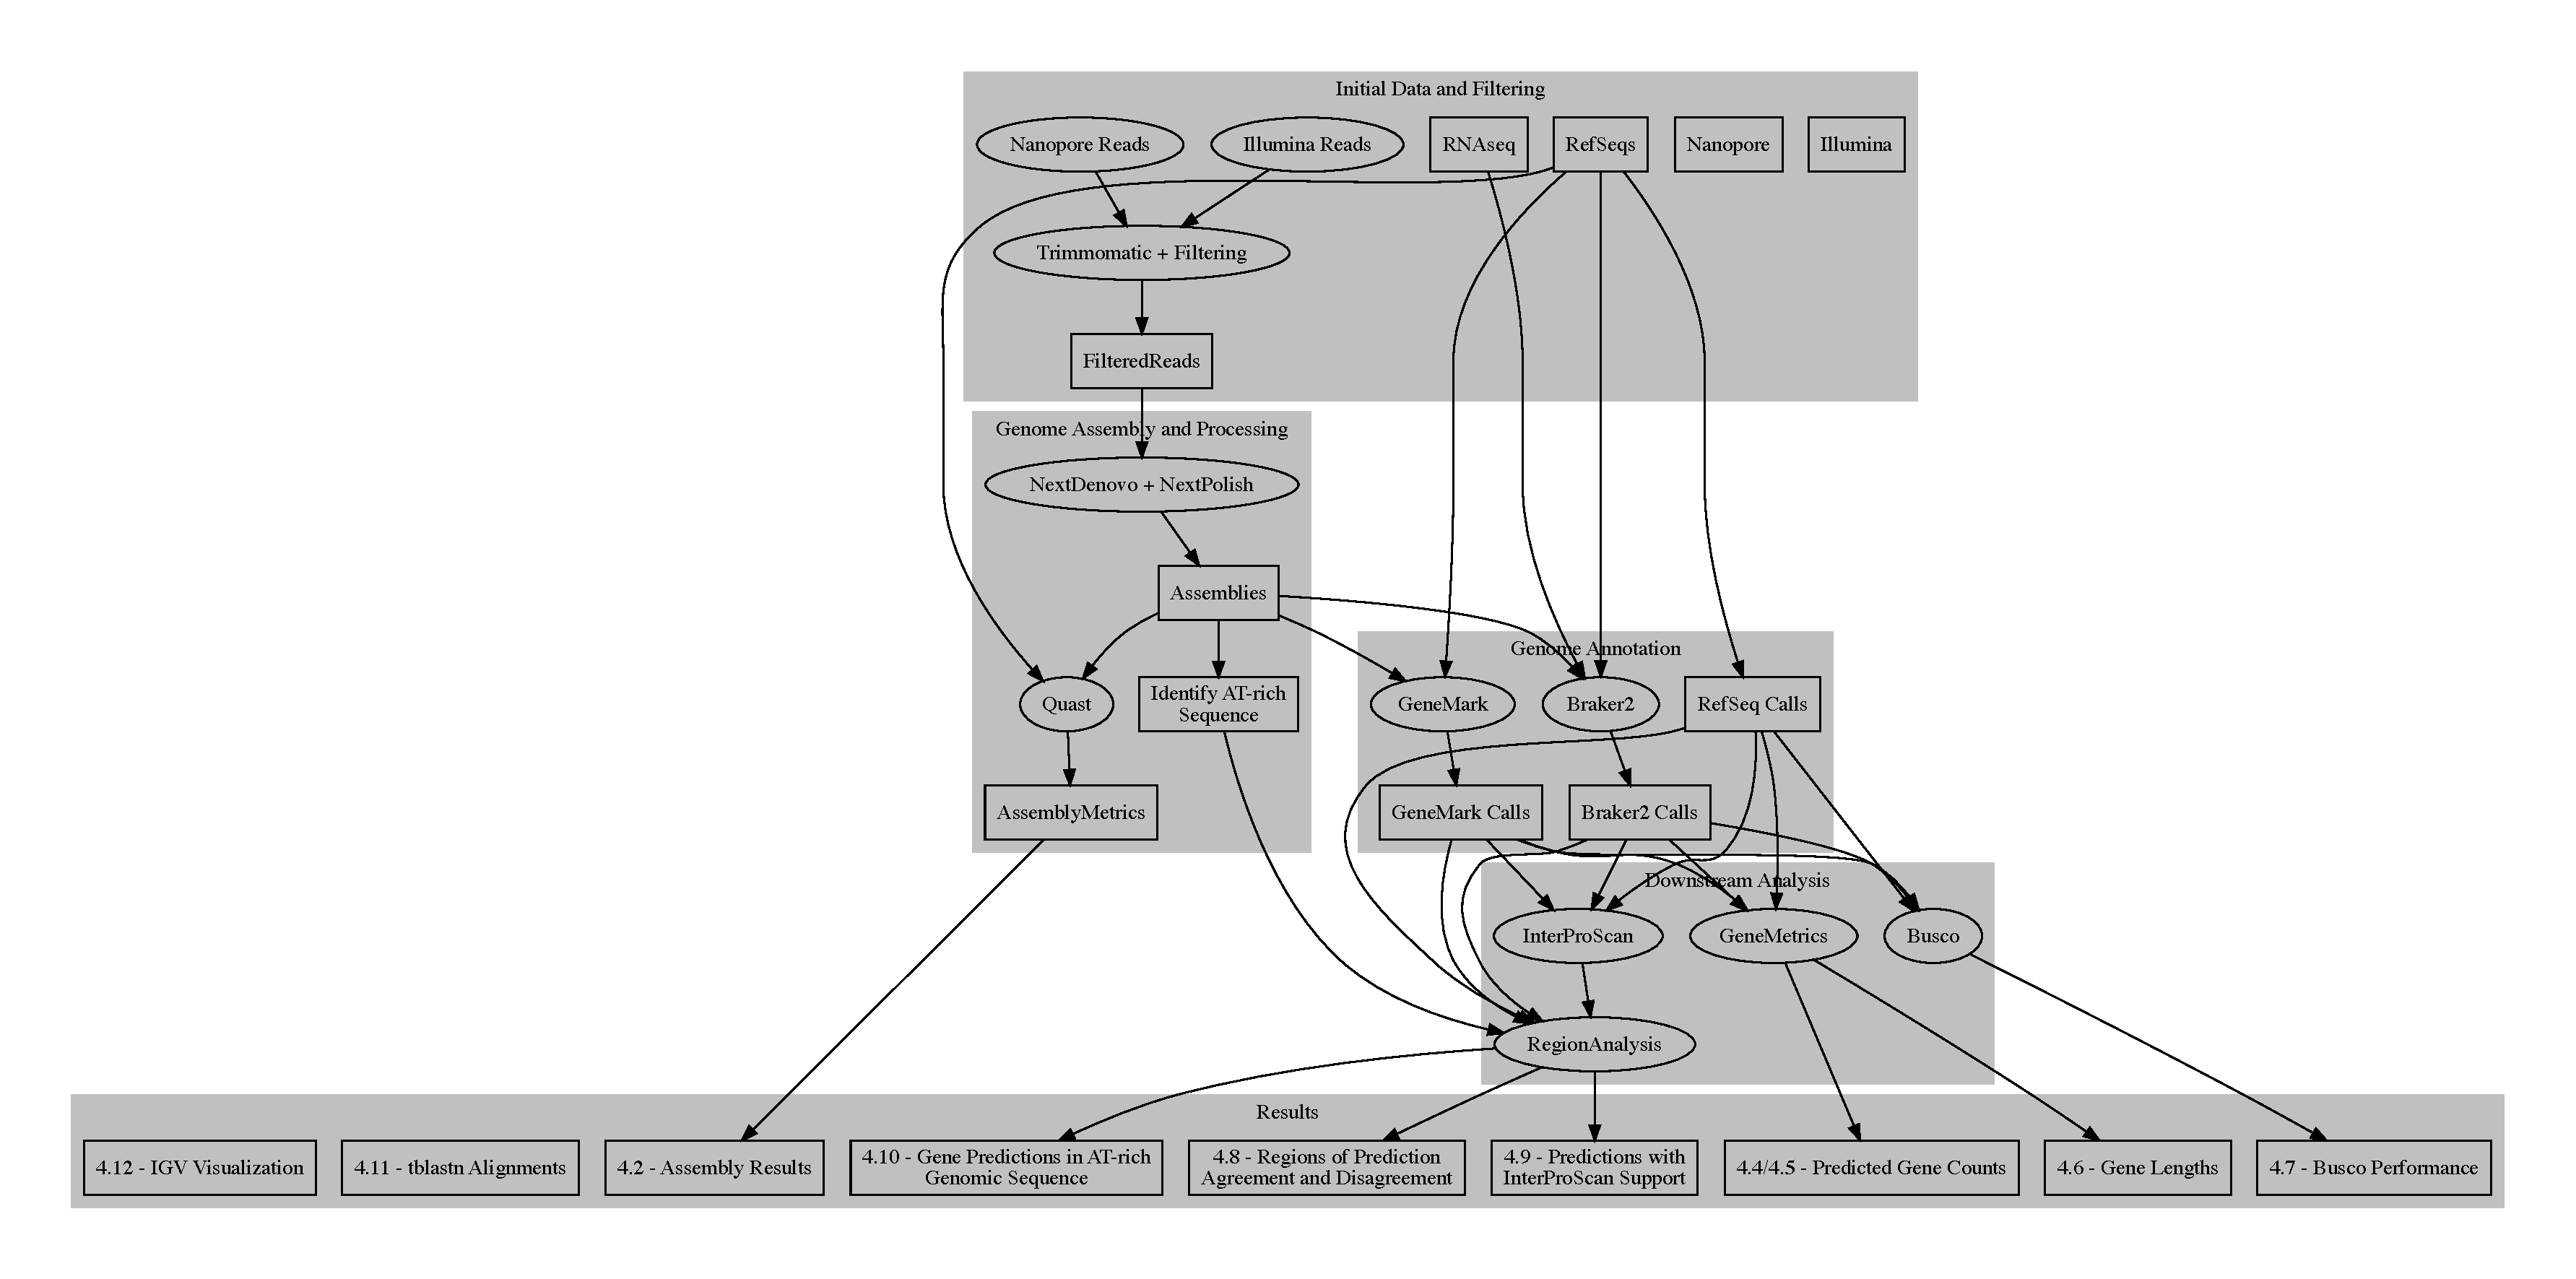
\includegraphics[width=1.25\textwidth]{./figures/data-flowchart.pdf}
%  }
%  \caption{A flowchart of the methodology followed in this
%    research. The workflow is broken up into sections based on the
%    processes and data involved at each step. Oval-shaped nodes
%    represent steps involved in the processing of data, while
%    rectangular nodes represent input and intermediate datasets as
%    well as results.}
%  \label{fig:workflow}
%\end{figure}

\section{Sequence Processing and Assembly Workflow}
\label{met:seq-workflow}

The sequence processing and assembly workflow is shown in Figure
\ref{fig:seq-workflow}. Processing steps are represented by boxes,
results of interest generated by this work are represented by folders,
and datasets that were not produced by this work are represented by
cylinders. Other workflows that use datasets produced by this workflow
are depicted as arrows outside of the brown subgraph.

Illumina\ref{Bennett2004} sequences were first trimmed and filtered
using Trimmomatic\cite{Bolger2014} to remove adapter content and
low-quality sequences. The processed Illumina sequences and
Nanopore\cite{Wang2021} sequences were then supplied to the hybrid
genome assembly tool NextDenovo\cite{Hu2024}. The processed Illumina
data was then used polish the assemblies with
NextPolish\cite{Hu2020}. Resulting assemblies were then analyzed to
identify AT-rich genomic sequence, analyzed with QUAST for general
assembly metrics, and finally supplied to the region identification
process.

The processing steps Trimmomatic filtering, NextDenovo assembly,
NextPolish Polishing and QUAST assembly assessment are described in
Section \ref{met:seq-process}. The AT-rich sequence identification
process is described later in Section \ref{met:atrich}.

\begin{figure}
  \centering
  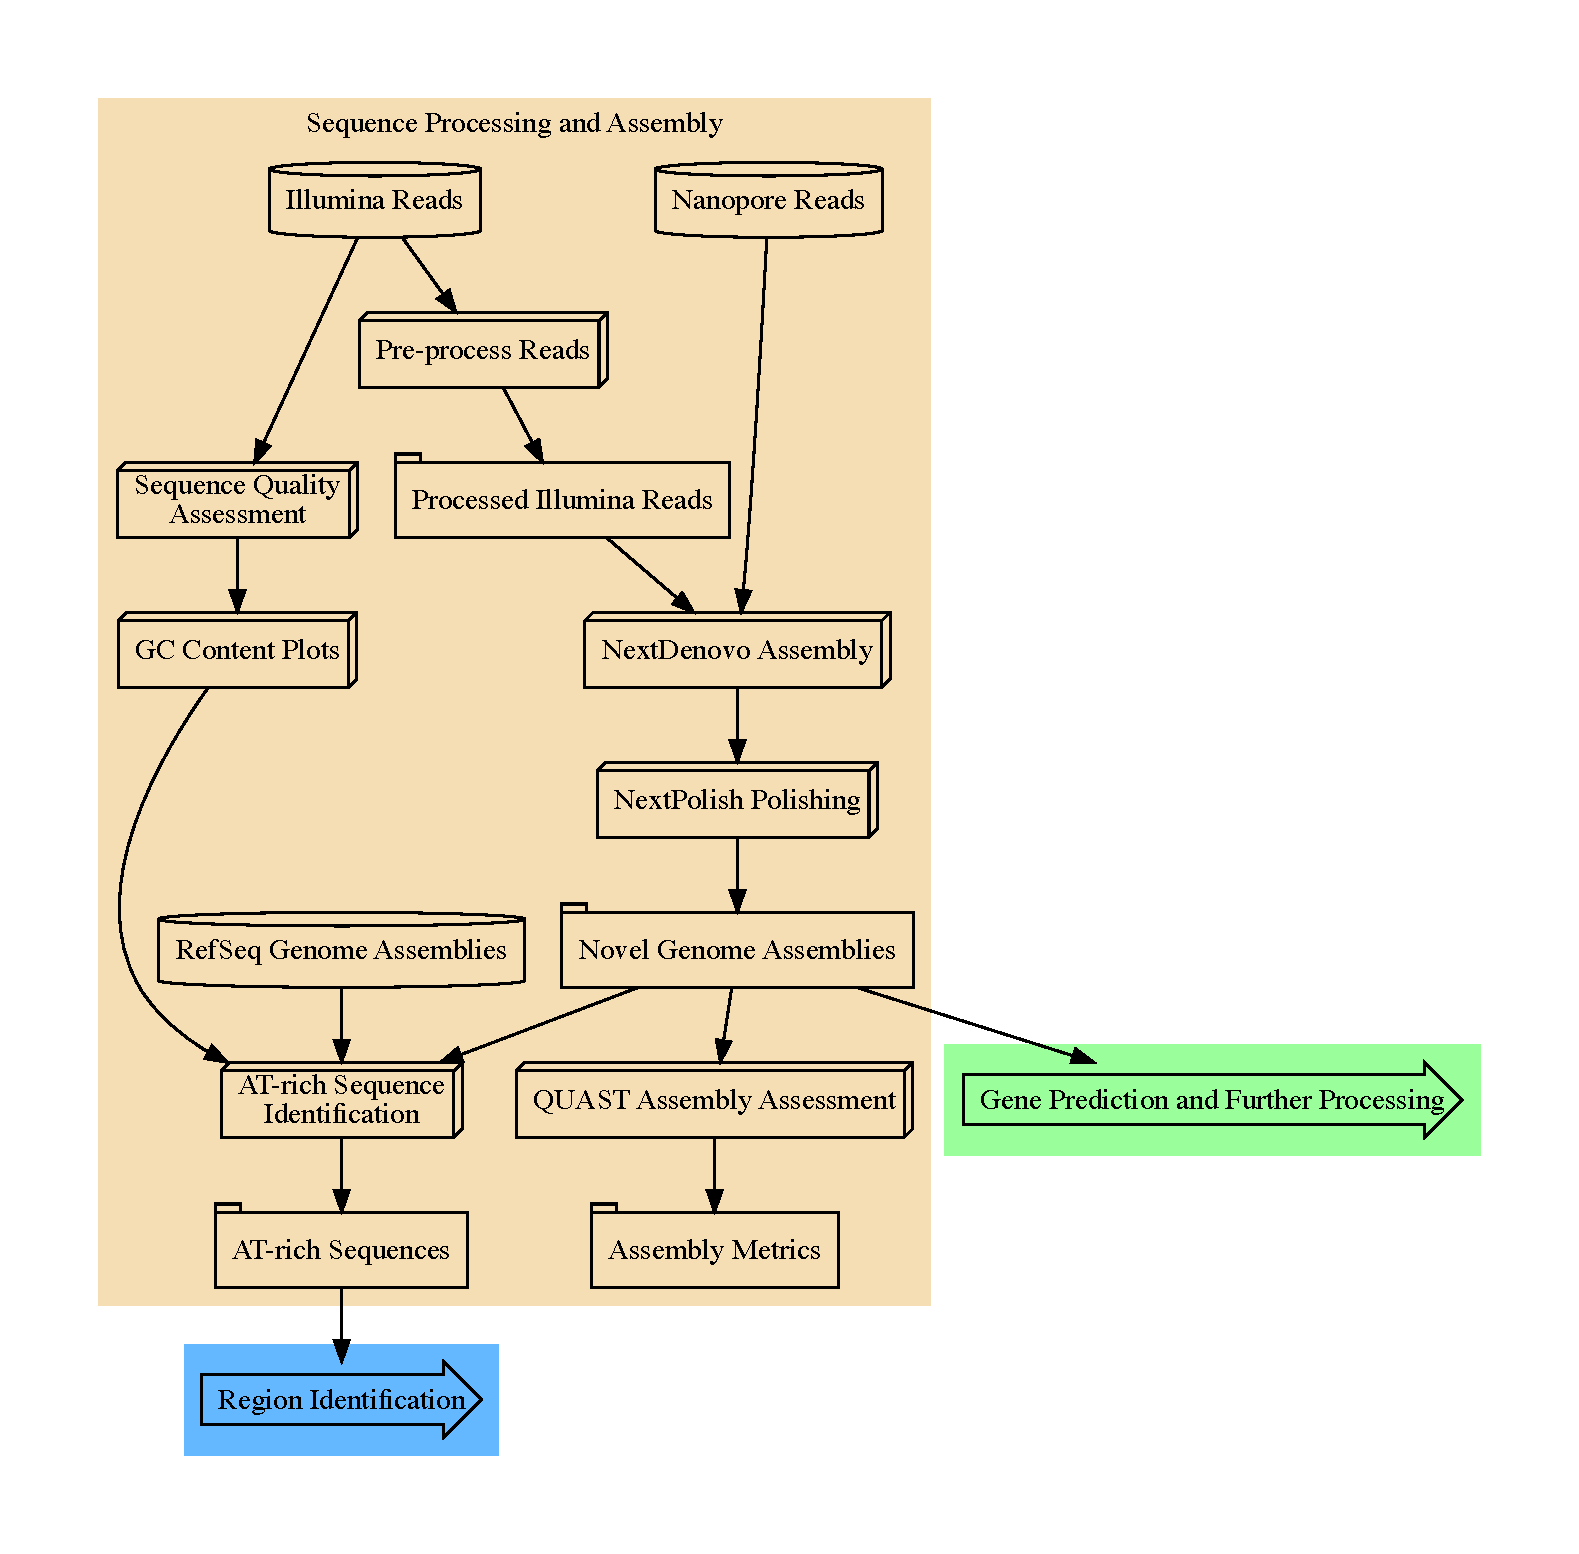
\includegraphics[width=\textwidth]{figures/assembly-met.pdf}
  \caption{A workflow (in brown) depicting the steps taken to process
    input sequences, generate assemblies, and post-process those
    assemblies for use in other workflows. Processing steps are
    represented by boxes, datasets of interest that were produced by
    this work are represented by folders, and datasets that were not
    produced in this work are represented by cylinders. Other
    workflows are represented by arrows outside of the brown
    subgraph.}
  \label{fig:seq-workflow}
\end{figure}

\section{Sequence Pre-processing and Assembly}
\label{met:seq-process}
% somewhere here...
% The training was performed using roughly 145 million Illumina
% paired end RNAseq reads on the \textit{Trichoderma reesei} genome.

Genomic sequences for assembling were generated for DC1 and Tsth20
using Nanopore\cite{Wang2021} and Illumina\cite{Bennett2004}
sequencing technologies by Brendan Ashby at the Global Institute for
Food Security at the University of Saskatchewan. Nanopore data was not
processed prior to assembly. Illumina sequencing data was filtered
using Trimmomatic v0.38\cite{Bolger2014} with filtering criteria as
follows: SLIDINGWINDOW:4:28, LEADING:28, TRAILING:28, MINLEN:75. Only
surviving paired-end reads were used for further analysis.

Genomic Nanopore sequences from DC1 and Tsth20 were assembled in to
contigs using NextDenovo\cite{Hu2024} v2.5.0 and then polished with
Illumina sequences using NextPolish\cite{Hu2020} v1.4.1. Assembly and
polishing were both performed using default parameters. Final assembly
metrics were calculated using QUAST v5.0.2\cite{Gurevich2013} with
default parameters.

%In an attempt to produce high quality assemblies of DC1 and Tsth20, We
%decided on a set of tools named NextDenovo and NextPolish as they have
%produced excellent assemblies based on previous experience. (should
%find a citation to confirm this)

%(Might be better for discussion or omitted since it is specific to our
%setup) Initial attempts to run the example dataset resulted in
%permissions errors due to the management of the storage system being
%used, which were encountered with other tools in the past. To remedy
%this, the software installation was copied to RSMI's scratch space on
%Copernicus. Once the approriate permissions were given to run
%nextDenovo, the example dataset was run without issue.

%Following assembly using nextDenovo, Illumina sequence data from DC1
%and Tsth20 was used to polish each respective genome using
%nextPolish. Default parameters were used from assembly except for
%modification of the parallel option to reduce processing times.

%\subsection{Repeat Masking}

%In order to evaluate the performance of gene finding tools in
%repetitive or low complexity regions in the context of
%\textit{Trichoderma} genomes, we must first identify said regions in
%the genomes considered. To do this, the GenericRepeatFinder tool was
%used, which is a \textit{de novo} repeat detection tool
%\cite{10.1104/pp.19.00386}. GenerifRepeatFinder detects three
%different types of repeats, those being MITEs, TDRs and TIRs. Commands
%used for this program follow the example commands provided on the
%GitHub page for the GenericRepeatFinder project.


\section{Gene Prediction and Further Processing}
\label{met:predict-workflow}

To better understand the methods used in gene prediction and CDS
analysis, the steps will be collected into several sub-workflows,
beginning with sequence processing and assembly as shown in Figure
\ref{fig:predict-workflow}. Processing steps are represented by boxes,
results of interest generated by this work are represented by folders,
and datasets that were not produced in this work are represented by
cylinders. Other workflows that use datasets produced by this workflow
are depicted as arrows outside of the green subgraph.

First, RefSeq assemblies and their associated annotations of closely
related \textit{Trichoderma} species were selected from NCBI for
training and comparison. Both and \textit{ab initio} (GeneMark\cite{Borodovsky2011}) and
evidence-based (Braker2\cite{Bruna2021}) gene finders were selected
for comparison to evaluate gene prediction behaviour in both scenarios
in the context of \textit{Trichoderma} genomes. Gene prediction was
performed using both gene finders on the RefSeq genomes and the
genomes of DC1 and Tsth20. Coding sequences (CDS) output by the gene
finders were then examined to better understand distributions of CDS
lengths produced by different gene finders. Finally, all gene
predictions were then supplied to the evaluation and validation stage
as well as the region identification stage.

Selection of NCBI datasets for training and comparison are further
discussed in Section \ref{met:datasets}. The GeneMark gene prediction
process is described in Section \ref{met:genemark}, while the Braker2
gene prediction process is described in Section \ref{met:braker2}. The
CDS processing step is described in Section \ref{met:cds-stats}.

\begin{figure}
  \centering
  \makebox[0pt]{
    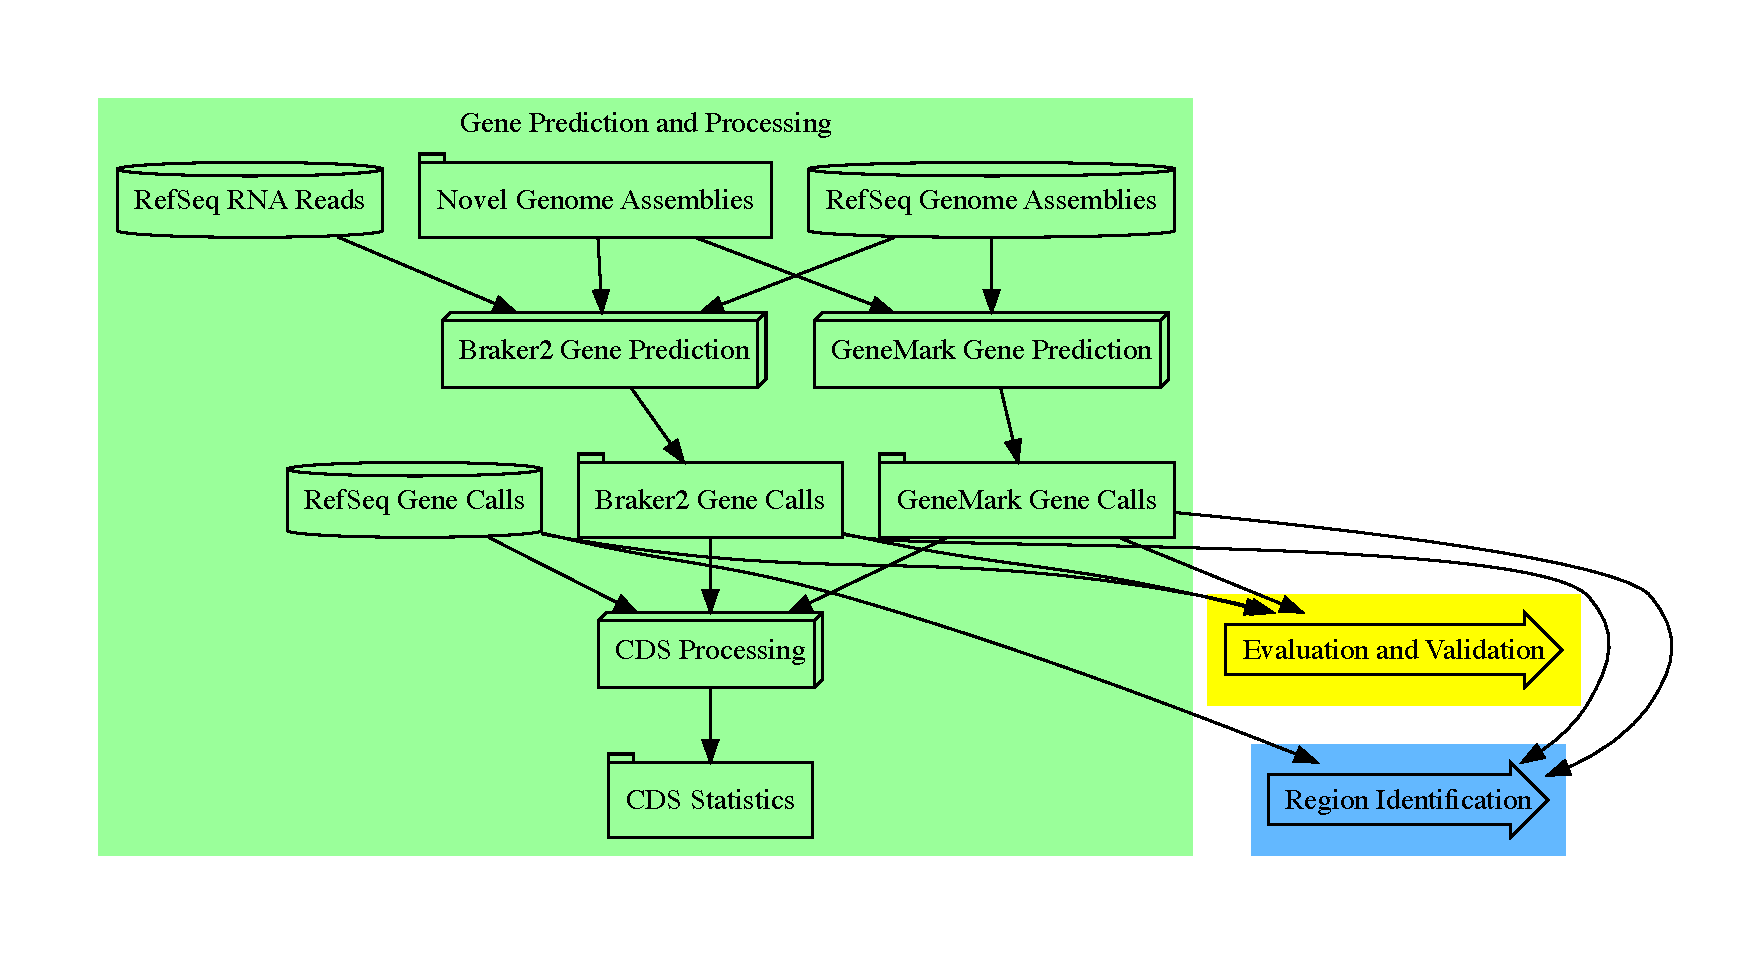
\includegraphics[width=1.15\textwidth]{figures/gene-finding-met.pdf}
  }
  \caption{A workflow (green) depicting the steps taken to predict
    genes for use in other workflows and process CDS sequence
    lengths. Processing steps are represented by boxes, datasets of
    interest that were produced by this work are represented by
    folders, and datasets that were not produced in this work are
    represented by cylinders. Other workflows are represented by
    arrows outside of the green subgraph.}
\end{figure}

\section{Selection of Datasets from NCBI}
\label{met:datasets}

It is important to evaluate gene finders in comparison to a standard
or control dataset as a method of ground-truthing. Such datasets
include reference genome sequences and their associated gene
predictions from NCBI. In addition to control datasets, RNAseq data
can also be used as training data for various tools as well, such as
the evidence-based training used by Braker2. In this work, four forms
of input were selected from NCBI for comparison and training. The
first two datasets are assemblies and associated gene predictions of
three RefSeq \textit{Trichoderma} accessions, with those accessions
being \textit{T. virens}, \textit{T. harzianum}, and
\textit{T. virens}. NCBI RefSeq accession IDs for those assemblies are
GCF\_000167675.1\_v2.0, GCF\_003025095.1\_Triha\_v1.0, and
GCF\_000170995.1\_TRIVI\_v2.0, respectively. \textit{T. reesei} was
selected as it is the most well-studied \textit{Trichoderma}
species. \textit{T. harzianum} and \textit{T. virens} were selected as
additional datasets due to their prevalence in literature as well.

The second set of inputs are RNAseq datasets from \textit{T. reesei},
used as input in the training process for Braker2. The SRA accession
IDs for those sequencing runs are: . Limited RNAseq datasets were used
as there were few RNAseq datasets were available at the beginning of
this project.

The final set of inputs are protein sequences from RefSeq individuals
\textit{T. atroviride}, \textit{Fusarium graminarium}, and
\textit{Saccharomyces cerevisiae}. The NCBI accession IDs for these
assemblies and associated protein sequences are GCF\_000171015.1,
GCF\_000240135.3, and GCF\_000146045.2, respectively.

\section{Gene Prediction Using GeneMark-ES}
\label{met:genemark}


\textit{Ab initio} gene finding was performed using GeneMark-ES
v4.71\cite{Borodovsky2011} with DC1, Tsth20 and selected RefSeq
\textit{Trichoderma} assemblies used as input. Default parameters were
used in all cases except for the fungal option, which was allowed the
use of a GeneMark model specific to fungal genomes.

%General command structure for GeneMark-ES:
%
%gmes\_petap.pl --ES --fungus
%--format gff3 --cores 48 --sequence /path/to/sequence

\section{Gene Prediction Using Braker2}
\label{met:braker2}

For evidence-based gene finding, Braker2 v3.0.2\cite{Bruna2021} was
used with \textit{Trichoderma reesei} selected as the reference
organism for training. RNAseq datasets from \textit{T. reesei} were
downloaded from the NCBI short-read archive using the
sra-toolkit\cite{NCBI2025} and were not trimmed or filtered prior to
their use in Braker2 training. Default parameters were used to train a
Braker2 model on \textit{Trichoderma reesei} data except in the case
of the fungal option, which was used for this analysis for improved
gene-finding performance in fungi. The trained Braker2
\textit{T. reesei} prediction model was then applied to all assemblies
with default parameters.

Braker2 also provides a UTR option to predict upstream sequence
features, but that option is experimental and was left off for this
work.

%The variables that need to be set are AUGUSTUS\_CONFIG\_PATH and
%TSEBRA\_PATH. Augustus, by defuault, tries to write species
%information to the location where the software is installed. In this
%case, we don'thave write permissions to the compute canada software
%stack hosted byt Research Computing, so the AUGUSTUS\_CONFIG\_PATH
%variable must be set in order to create a writeable directory. As long
%as that path has a directory within it called braker, and a species
%directory within the braker directory, things should go
%smoothly. TSEBRA is a set of scripts also made by the creators of
%Braker and is required to merge results from the various gene
%prediction tools involved in the Braker2 pipeline. The TSEBRA\_PATH
%simply points to the directory where TSEBRA is located Both Braker2
%and TSEBRA can be cloned directly from GitHub (links to come)

\section{Statistical Analysis of CDS Lengths}
\label{met:cds-stats}
The distribution of gene lengths predicted by a gene-finder is an
important feature to consider when selecting a gene finding tool, as
genes of a particular length may be of interest to researchers, but
more importantly, gene-finders may be biased to certain distributions
based on their underlying models. These biased distributions may
differ from the true distribution of CDS lengths leading to
propagation of sub-optimal gene-finding results. To determine, at
minimum, if differences exist between distributions of predicted gene
lengths from each tool, the $log^10$ lengths of coding sequences (CDS)
were subject to a two-sample Kolmogorov-Smirnov test\cite{ref1}. 

\section{Evaluation and Validation of Gene Predictions}
\label{met:valid-workflow}

Following the gene prediction process, prediction results can then be
evaluated and queried against exiting datasets as a form of
validation. The workflow for evaluation and validation of gene
predictions if shown in Figure \ref{fig:valid}. Processing steps are
represented by boxes, results of interest generated by this work are
represented by folders, and datasets that were not produced in this
work are represented by cylinders. Other workflows that use datasets
produced by this workflow are depicted as arrows outside of the yellow
subgraph.

Coding sequences from the previous stage were then evaluated and
validated using several tools. Firstly, protein products from
predicted CDSs were processed with InterProScan to identify Pfam
domains as evidence for the validity of gene predictions. Secondly,
CDSs were analyzed with BUSCO to assess prediction of conserved fungal
genes. Finally, 

BUSCO evaluation, InterProScan Annotation, and BLAST alignment
processes are described in more detail in Sections \ref{met:busco},
\ref{met:interproscan}, and \ref{met:blast}, respectively. Results
from these processes are also used as inputs in the region
identification workflow later.

\begin{figure}
  \centering
  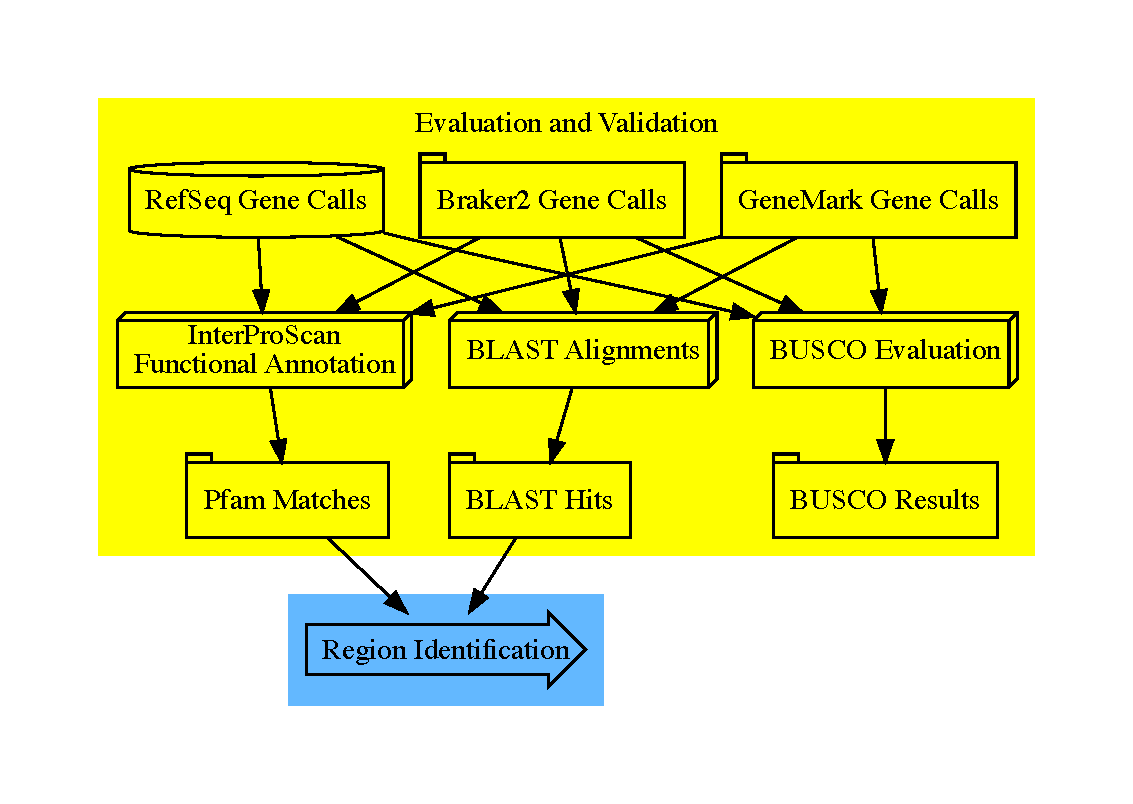
\includegraphics[width=0.8\textwidth]{figures/eval-met.pdf}
  \caption{A workflow (yellow) depicting the steps taken to evaluate
    and validate predicted genes. Processing steps are represented by
    boxes, datasets of interest that were produced by this work are
    represented by folders, and datasets that were not produced in
    this work are represented by cylinders. Other workflows using
    results from these processing steps are represented by arrows
    outside of the green subgraph.}
  \label{fig:valid}
\end{figure}

\section{Evaluating Gene-Finder Performance Using BUSCO}
\label{met:busco}
While novel gene predictions are of great interest in new subjects, it
is also important to confirm that gene-finders are predicting genes
that are expected to be present in the organism of
interest\cite{https://doi.org/10.1002/cpz1.323}. To determine if this
is true, BUSCO v5.7.1\cite{10.1093/bioinformatics/btv351} was selected
as a tool to determine a gene-finder's ability to predict a set of
conserved ortholagous genes. The BUSCO Metaeuk pipeline was run using
the BUSCO fungi\_Odb10 fungal lineage dataset to capture highly
conserved genes in fungal genomes. This pipeline was applied to all
genome assemblies used in this work. (note for us to discuss: I used
transcriptome mode...)

\section{Functional Annotation Using InterProScan}
\label{met:interproscan}
The predicted proteins from each gene finder were functionally
annotated using InterProScan
v5.65-97.0\cite{10.1093/bioinformatics/btu031} without the match
lookup service and with the following analyses included: AntiFam-7.0,
CDD-3.20, Coils-2.2.1, FunFam-4.3.0, Gene3D-4.3.0, Hamap-2023\_01,
MobiDBLite-2.0, NCBIfam-13.0, PANTHER-18.0, Pfam-36.0, PIRSF-3.10,
PIRSR-2023\_05, PRINTS-42.0, ProSitePatterns-2022\_05,
ProSiteProfiles-2022\_05, SFLD-4, SMART-9.0,
SUPERFAMILY-1.75. InterProScan was run on all predicted proteins using
default parameters. The resulting protein annotations were mapped back
to the gene predictions and processed using the region identification
algorithm in section \ref{section:region-met}.

\section{Ground-truthing with BLAST}
\label{met:blast}
The \textit{Trichoderma} assemblies chosen for comparison were used as
the subject sequences in tblastn searches with the query proteins
discussed in paragraph three of Section \ref{met:datasets}. Default
parameters were used in the tblastn searches. Hits from the tblastn
alignments were then filtered for alignments with a minimum of 30\%
query coverage and 30\% identity. These criteria were selected as they
filter out spurious alignments while also retaining short alignments
that capture functional or conserved protein coding
sequence. Remaining aligments were then converted to GFF format and
processed using the region identification algorithm in
\ref{section:region-met}

\section{Region Identification Overview}
\label{section:region-overview}
A major portion of this work was the process of identifying regions of
overlapping features as a method of comparing gene calls from
different assemblers. The definition of a region and the algorithm
used to identify them is described in detail in Section
\ref{section:region-met}, and an overview of the region identification
workflow is shown in Figure \ref{fig:region-overview}. The top of the
graph shows the gene calls produced by the workflow described in
Section \ref{met:predict-workflow}, which are used as input in along
with other previously generated datasets. These additional datasets
may contain other information such as blast alignments or functional
annotation can be included as features in the region identification
process. Datasets outlined with rectangles indicate that the data
within were processed with the input gene calls and discussed in their
own results sections. Datasets output by the region identification
process were then visualized with the Integrative Genomics Viewer,
described in Section \ref{section:igv-met}

\begin{figure}
  \centering
  \makebox[0pt]{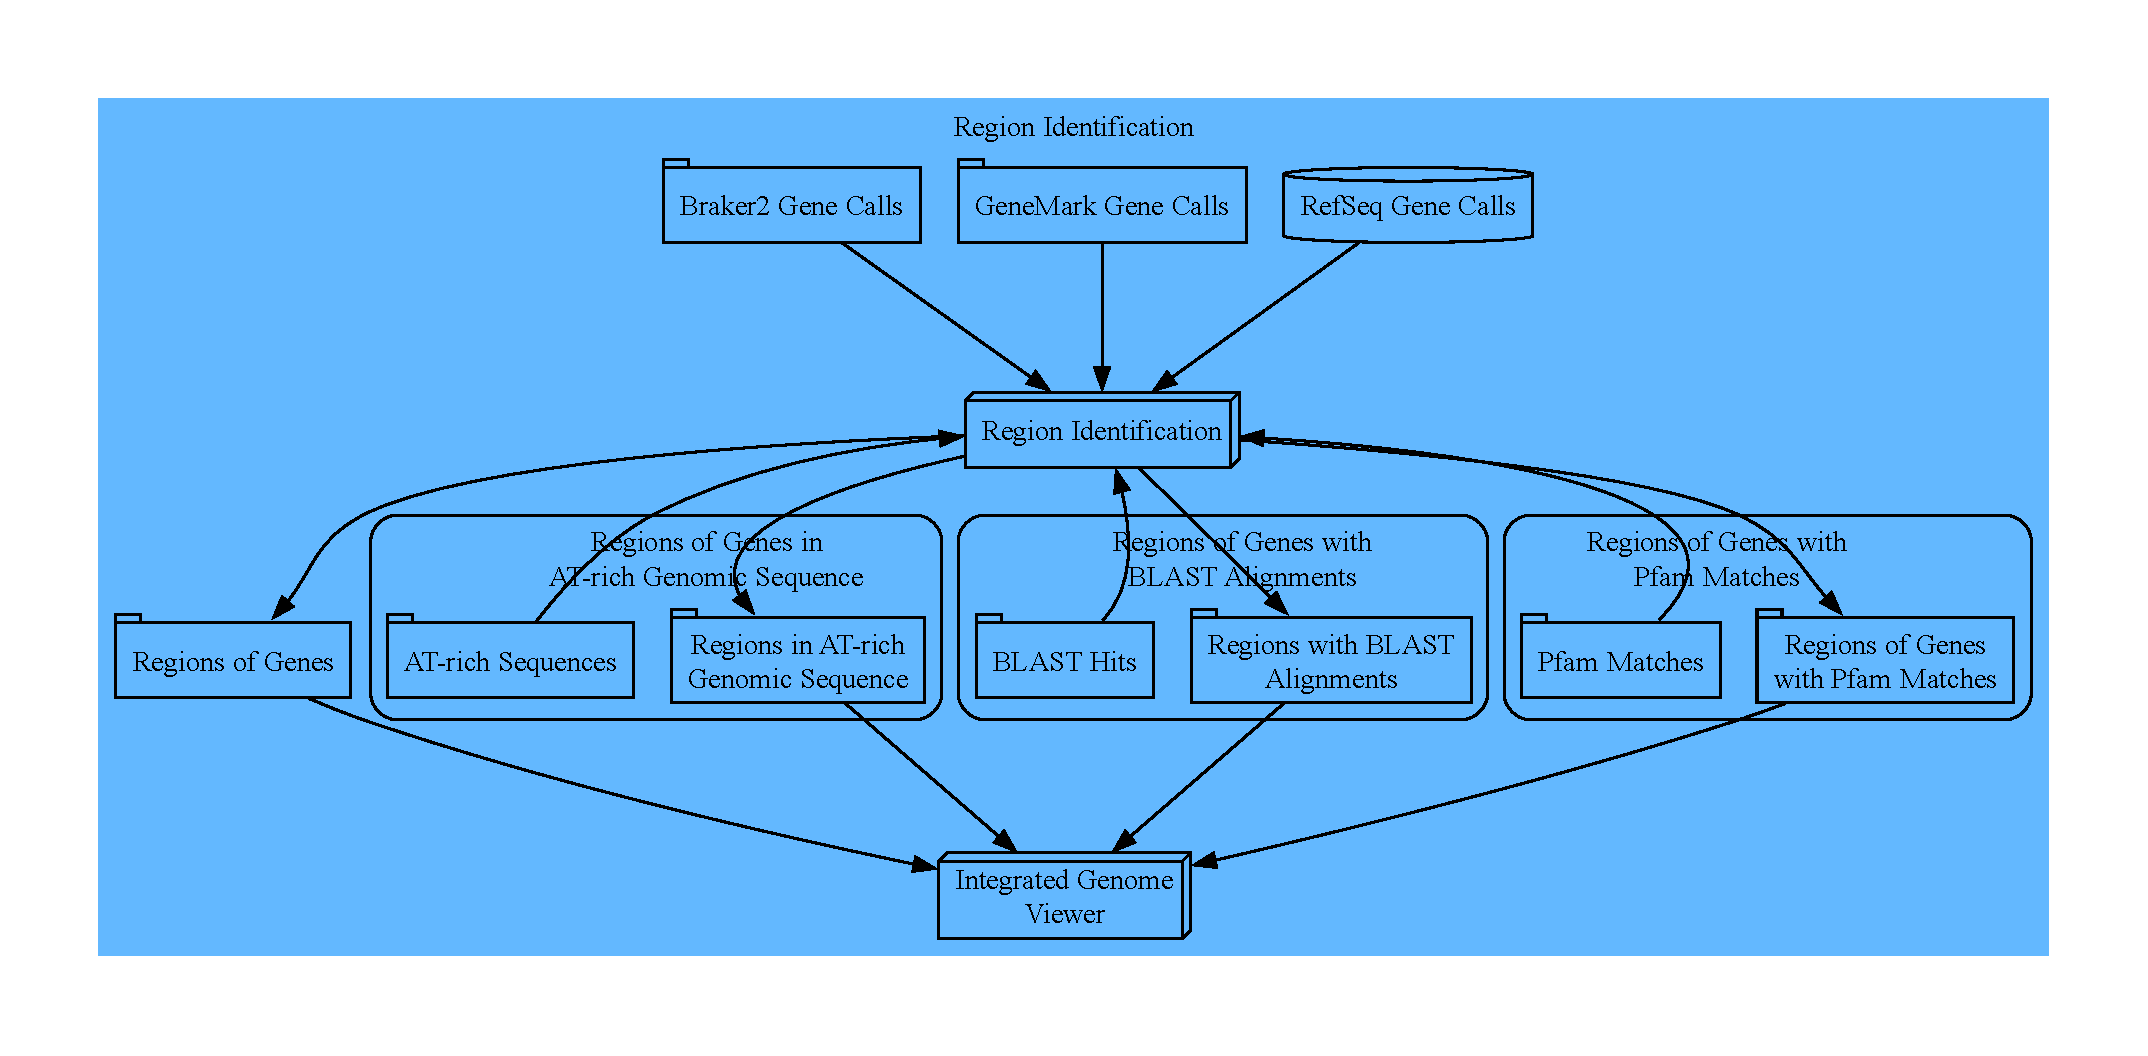
\includegraphics[width=1.2\textwidth]{figures/region-workflow.pdf}}
  \caption{An overview of the region identification process for
    different datasets. Sections of the graph are outlined with
    rectangles, indicating that the datasets within were processed
    along with gene calls and discussed in their own results
    sections. Processing steps are represented by boxes, datasets of
    interest that were produced by this work are represented by
    folders, and datasets that were not produced by this work are
    represented by cylinders.}
  \label{fig:region-overview}
\end{figure}


\section{Region Identification Algorithm}
\label{section:region-met}

Predictions and results from \ref{met:genemark} and \ref{met:braker2}
were processed into regions of overlapping gene predictions and
annotations. A region is defined as a pair of start and stop genomic
coordinates which contains one or more overlapping features. We define
a feature as a set of start and stop positions associated with a
single gene prediction, annotation or other data point of interest.

Overlapping features were processed into regions using a concept
similar to Allen's interval algebra\cite{DECHTER2003333}. The
algorithm first sorts all features on each contig by start coordinate
and then iterates over each feature, identifying overlaps with
previous features to identify regions of overlapping
features. Pseudocode for the algorithm is shown in algorithm
\ref{alg:regions}. This processing was performed with Python
v3.12.4\cite{Foundation} and the GFF package from BCBio\cite{Chapman}
for easy GFF parsing.  The resulting regions were then further
processed to identify trends and behaviours of gene finders in the
context of other annotated information and features.

\begin{algorithm}
  \begin{algorithmic}
    \State INPUT:\ list\ of\ GFF\ files,\ $GFFList$
    \State RETURNS:\ list\ of\ regions,\ $regionList$
    \For{\texttt{<each GFF in GFFList>}}
    \State $allFeatures \gets GFF.features$
    \EndFor
    \State $sortedFeatures \gets sortStartCoord(allFeatures)$
    \State $regionList \gets []$
    \State $firstFeature \gets firstItem(sortedFeatures)$
    \State $lastFeature \gets lastItem(sortedFeatures)$
    \For{\texttt{<each feature in sortedFeatures>}}
      \If{$feature = firstFeature$}
        \State $currentRegion \gets newRegion(feature)$
        \State $currentRegion.start \gets feature.start$
        \State $currentRegion.end \gets feature.end$
      \ElsIf{$feature = lastFeature$}
        \State $regionList.append(currentRegion)$
        \State $return\ regionList$
      \ElsIf{$feature\ overlaps\ currentRegion$}
        \State $currentRegion.updatePositions(currentRegion, feature)$
        \State $currentRegion.addFeature(feature)$
      \Else
        \State $regionList.append(currentRegion)$
        \State $currentRegion \gets newRegion(feature)$
        \State $currentRegion \gets feature.start$
        \State $currentRegion \gets feature.end$
      \EndIf
    \EndFor
    \State $return\ regionList$
  \end{algorithmic}
  \caption{The general algorithm underlying the region identification
    process.}
  \label{alg:regions}
\end{algorithm}

\section{Gene predictions in AT-rich Genomic Sequence}
\label{met:atrich}
AT-rich genomic sequences were identified using sliding windows of GC
content over each \textit{Trichoderma} assembly. Sliding windows were
generated using the isochore program from the EMBOSS tool suite
v6.6.0\cite{Rice2000}. The sliding window used was 250bp wide with a
50bp shift. A window was classified as AT-rich if the sequence
contained lower than 28\% GC content. The genomic sequences from
AT-rich windows were mapped to a GFF file and processed using the
region identification algorithm described in section
\ref{section:region-met}.

\section{Visualization of Identified Regions}
\label{section:igv-met}
Results from the region identification process were visualized using
the IGV genome browser v2.19.1\cite{Robinson2011}. An example of an
IGV screenshot is shown in Figure \ref{fig:igv-methods}

\begin{figure}
  \centering
  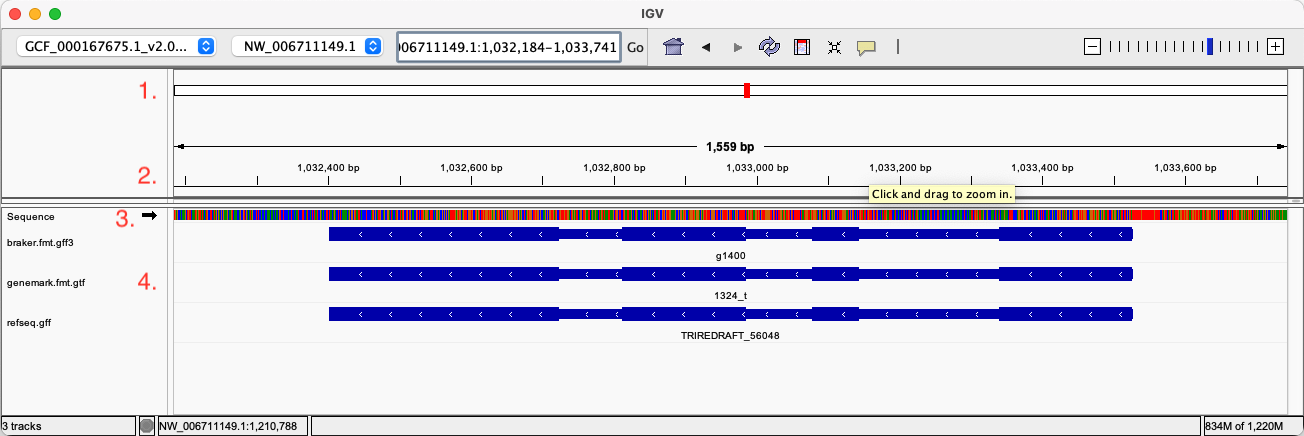
\includegraphics[width=0.9\textwidth]{figures/igv/igv-agreement-thin-number}
  \caption[IGV example]{An example of an IGV screenshot used in
    portions of the results from this work. The top half of the image
    displays information about the reference sequence with box one
    showing the position of the viewer relative to the reference
    sequence, and box two showing the numerical positions of the
    reference. The lower half of the image displays tracks, or
    additional layers of information mapped to the reference
    sequence. Box three shows a track displaying the nucleotide at
    each position if the scale of the viewer is small enough. Box four
    shows several tracks, each containing features, the regions in
    blue, from a GFF file. The tracks in this example are limited to
    gene predictions, although tracks in other IGV screenshots may
    include features from other tools such as InterProScan. Individual
    tracks will be referred to in increasing numerical order in the
    track list beginning from the top. The nucleotide track is not
    included in the order.}
  \label{fig:igv-methods}
\end{figure}

%=======
%Example command for braker2:
%
%/scratch/p2irc/p2irc\_rsmi/cbe453/masters/software/braker2/BRAKER/scripts/braker.pl
%--gff3 --threads 60
%--TSEBRA\_PATH=/scratch/p2irc/p2irc\_rsmi/cbe453/masters/software/braker2/tsebra/TSEBRA/bin/
%--genome /path/to/sequence --species=TreeseiFungal --fungus
%--useexisting
%
%BUSCO methodology (from research questions)
%The BUSCO method was applied using two BUSCO subsets,
%one generally applicable for fungi, and another targeting an
%evolutionary branch more closely related to \textit{Trichoderma}.
%
%Stats for length analysis (from research questions)
%The first statistical tool to be applied is ANOVA (analysis of
%variance) to compare the mean lengths genes predicted by each gene
%finding tool with the null hypothesis being that the mean of predicted
%gene lengths should be the same across all tools considered. In
%addition to ANOVA, pairwise comparisons of the distributions using a
%Kolmogorov–Smirnov test is appropriate. The null hypothesis in this
%test would be that the gene lengths are sample from the same
%distribution.
%
%Stats for binomial tests (from research questions)
%To do this, a binomial test will be used, with the null hypothesis
%being that the number of genes predicted in regions of normal and
%abnormal GC content should be proportional to the length of normal and
%abnormal GC content regions in the assembly. For example, if 30
%percent of the genome is comprised of anomalous GC content, then we
%would expect 30 percent of predicted genes to be present in those
%regions. In addition to anomalous GC content, this test can be applied
%to repetitive content in assemblies as well.
%
%Stats for regions (from research questions)
%From these results, Venn diagrams will be generated with
%Jaccard index calculated for each combination of gene finding
%tools. The region identification process can also be extended to
%include features identified by other tools, such as BLAST hits to
%validated gene models from other organisms and small RNAs. Chi2
%goodness of fit tests can then be applied to counts of 'validated'
%gene predictions or other features with the same null hypothesis that
%gene finders should predict the same number of features.
